\chapter{Mean Shift Algorithm Analysis} % (fold)
\label{cha:algorithm_analysis}
Before any porting can be started the developer has to find out if there are 
multiple activities or tasks which run simultaenously to expose exploitable 
concurrency. The developer has to find concurrency either by decomposing the  
data or tasks. By this decomposition one wants to solve bigger problems in less 
time as several processing units can solve different parts of the problem. 

But before any analysis is started one has to know if the problem is large enough
and if the resulting speedup justifies all the effort that is expended on making
a parallel version out of it. In case of mean shift which is used for several 
things like filtering, segmentation, pattern recognition and real time tracking
one can deduce that for bigger images or many images the computation time climbs
fast as the size or the number of images rises. To have a clue how the mean 
shift algorithm behaves with big pictures several run times where recorded.
For the analysis of the mean shift algorithm a ready to use \gls{EDISON} 
was used that was profiled and modified and parallelized for the purpose of this 
thesis.

The
\gls{EDISON}\footnote{http://www.caip.rutgers.edu/riul/research/code/EDISON/index.html}
system which was developed by the authors  \citeauthor{citeulike:462300} of
\citep{citeulike:462300} offers functionality to filter, segment and detect
edges in images. 

The \autoref{fig:cpu_run_time}
shows results of \gls{CPU} run times of the \gls{EDISON} application dependant
on image size. The vertical axis shows the run time in seconds and the
horizontal axis shows the side length in pixels of the quadratic \autoref{fig:orig0}.

\begin{figure}[ht]
\centering
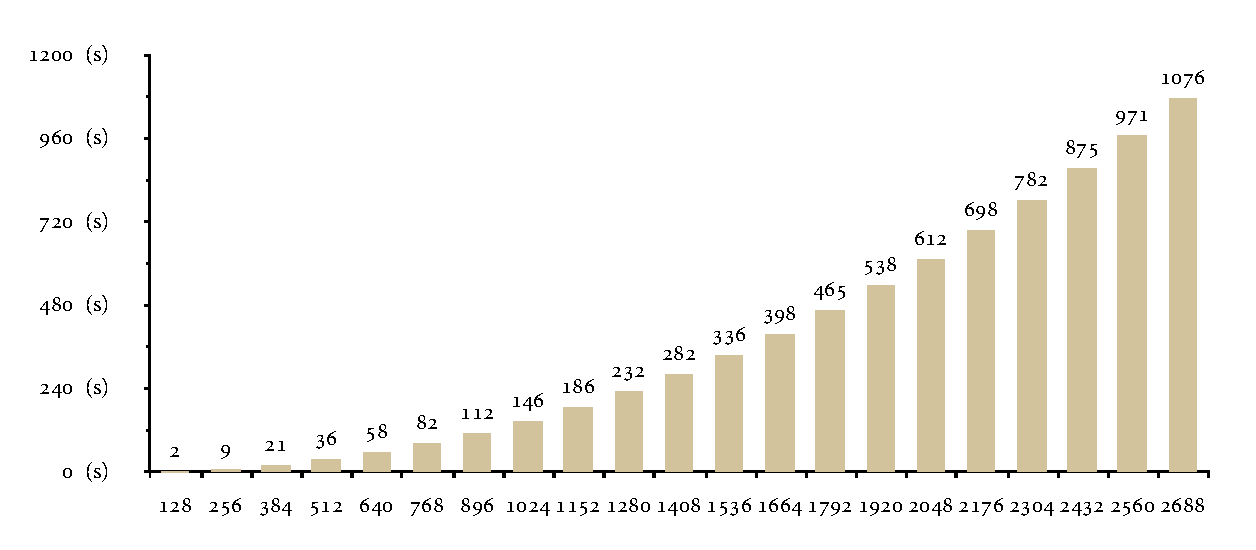
\includegraphics[width=390pt]{gfx/cpu_run_time}
\caption{CPU run time depending on the image size}
\label{fig:cpu_run_time}
\end{figure}




\section{Profiling the Original Code} % (fold)
\label{sec:run_time_analysis_of_the_original_code}
The first step before any porting to the \gls{GPU} is undertaken one has to
identify the portions of code that can be optimized. The procedure is called
profiling. In this case a statistical profiler is used which operates by
sampling. The samples are taken from the hardware performance counters which
every modern \gls{CPU} has builtin. OProfile a system wide profiler for Linux
was used to examine the run time of the \gls{EDISON} program.

The \autoref{tab:comp} shows the run time analysis of \gls{EDISON}. 


\begin{table}[ht]
   \myfloatalign
	\rowcolors{2}{gray!10}{}
  \begin{tabularx}{\textwidth}{cclcc} \toprule
    \tableheadline{Self} & 
	\tableheadline{Total} & 
	\tableheadline{Symbol} &
	\tableheadline{Size} &
	\tableheadline{Module}\\ \midrule
	0,0\% &	100,0\% &	main &											589B & edison \\  
	0,0\% & 	100,0\% & 	Run(CmCParser*) &								576B & 	edison \\ 
	0,0\% & 	100,0\% & 	EXECUTE(int, CmCParser*, void**) &				1,24KB &	edison \\ 
	0,0\% & 	100,0\% & 	EDISON::Segment() &								27B & 	edison \\
	0,0\% & 	100,0\% & 	EDISON::meanShift(int) &							2,75KB & edison \\ 
	\color{seccolor}0,0\% & \color{seccolor}99,3\% & 
	\color{seccolor}msImageProcessor::Filter(...) & 
	\color{seccolor}676B & \color{seccolor}edison \\
	0,4\% & 	99,1\% & 	msImageProcessor::NonOptimizedFilter(...) &		1.007B & edison \\ 
	0,6\% & 	98,8\% & 	MeanShift::LatticeMSVector(double*, double*) &	250B & 	edison \\ 
	98,2\% & 	98,2\% & 	MeanShift::uniformLSearch(double*, double*) & 	1,01KB & edison \\ 
	0,0\% & 	0,4\% & 	msImageProcessor::FuseRegions(float, int) &		1,17KB & edison \\ 
	0,1\% & 	0,3\% & 	msImageProcessor::BuildRAM() &					2,29KB & edison \\ 
	0,0\% &	0,2\% & 	msImageProcessor::TransitiveClosure() &			1,63KB & edison \\
	0,0\% & 	0,2\% & 	msImageProcessor::Prune(int) &					1,56KB & edison \\ 
	0,0\% & 	0,2\% & 	msImageProcessor::GetResults(unsigned char*) & 	340B & 	edison \\
	0,1\% & 	0,2\% & 	msImageProcessor::LUVtoRGB(...) &				542B & 	edison \\
	0,2\% & 	0,2\% & 	RAList::Insert(RAList*) &						249B & 	edison \\
	0,0\% & 	0,1\% & 	msImageProcessor::DefineImage(...) &				356B & 	edison \\
	0,1\% & 	0,1\% & 	msImageProcessor::RGBtoLUV(...) &				556B & 	edison \\
	0,0\% & 	0,1\% & 	msImageProcessor::Connect() &					455B & 	edison \\
	0,1\% & 	0,1\% & 	msImageProcessor::Fill(int, int) & 				440B & 	edison \\
	0,1\% & 	0,1\% & 	msImageProcessor::InWindow(int, int) & 			372B &	edison \\
	0,0\% & 	0,0\% &	msImageProcessor::GetBoundaries() &				39B & 	edison \\
	0,0\% & 	0,0\% & 	msImageProcessor::SqDistance(int, int) & 			256B & 	edison \\ 
	0,0\% & 	0,0\% & 	msImageProcessor::DefineBoundaries() &			1,41KB & edison \\ 
    \bottomrule
  \end{tabularx}
  \caption[EDISON run time profile]{\gls{EDISON} run time analysis}
  \label{tab:comp}
\end{table}




